

%-------------------------------------------------------------------------------
% Dokumenten Klasse
\documentclass[
	final,
	a4paper,
	oneside,
	parskip=full,
	headings=standardclasses,
	headings=big,
	pointednumbers
]{scrartcl}

%-------------------------------------------------------------------------------
% Packete nutzen
\usepackage{ngerman,palatino,setspace}
\usepackage[T1]{fontenc}
\usepackage[utf8]{inputenc}
\usepackage[left=20mm,right=20mm,top=25mm,bottom=25mm]{geometry}
\usepackage{amsmath}
\usepackage{mathtools}
\usepackage{tikz}

\usetikzlibrary{automata, positioning, arrows, calc}

%{
%\tikzset{
%    ->, % makes the edges directed
%    >=stealth, % makes the arrow heads bold
%    node distance=2cm, % specifies the minimum distance between two nodes. Change if necessary.
%    every state/.style={thick, fill=gray!10}, % sets the properties for each ’state’ node
%    every edge/.append style={line width=0.25mm}, % sets the properties for each ’state’ node
%    initial text=$ $, % sets the text that appears on the start arrow
%}
%}

\tikzset{
    node distance=2cm, % Minimum distance between two nodes. Change if necessary.
    every state/.style={ % Sets the properties for each state
        semithick,
        fill=gray!10
    },
    initial text={}, % No label on start arrow
    double distance=2pt, % Adjust appearance of accept states
    every edge/.style={ % Sets the properties for each transition
        draw,
        ->,>=stealth, % Makes edges directed with bold arrowheads
        auto,
        semithick
    }
}

%-------------------------------------------------------------------------------
\usepackage{multirow}

%-------------------------------------------------------------------------------
% uline
\usepackage{ulem}

%-------------------------------------------------------------------------------
% Anderer Font
\usepackage{mathrsfs}
\usepackage[mathcal]{euscript}

%-------------------------------------------------------------------------------
% Square brackets
\usepackage{stmaryrd}

%-------------------------------------------------------------------------------
% Dokument
\begin{document}
    
    
    %--- Page 1 --------------------------------------------------------------------
    
    $\Sigma = \left\{ \; a, b \; \right\} $ \quad
    $R = `` \left( \; ab \cup a \; \right)^* "{} $ \quad
    $\mathscr{L} = \llbracket \; \left( \; ab \cup a \; \right)^* \; \rrbracket $
    
    \begin{minipage}{0.1\textwidth}
        $a$:
    \end{minipage}
    \begin{minipage}{0.9\textwidth}
        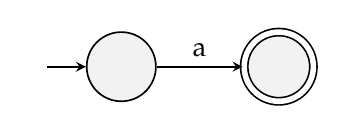
\begin{tikzpicture}
            \node[state, initial left]                  (q1)    {};
            \node[state, accepting, right of=q1]        (q2)    {};
            \draw   (q1) edge[]         node{a} (q2)
            ;
        \end{tikzpicture}
    \end{minipage}
    
    \begin{minipage}{0.1\textwidth}
        $b$:
    \end{minipage}
    \begin{minipage}{0.9\textwidth}
        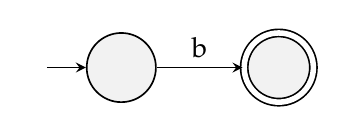
\begin{tikzpicture}
            \node[state, initial left]                  (q1)    {};
            \node[state, accepting, right of=q1]        (q2)    {};
            \draw   (q1) edge[]         node{b} (q2)
            ;
        \end{tikzpicture}
    \end{minipage}
    
    \begin{minipage}{0.1\textwidth}
        $ab$:
    \end{minipage}
    \begin{minipage}{0.9\textwidth}
        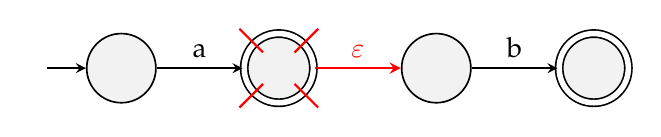
\begin{tikzpicture}
            \node[state, initial left]                  (aq1)   {};
            \node[state, accepting, right of=aq1]       (aq2)   {};
            \node[state, right of=aq2]                  (bq1)   {};
            \node[state, accepting, right of=bq1]       (bq2)   {};
            \coordinate (x) at (aq2);
            \draw   (aq1) edge[]        node{a} (aq2)
                    (bq1) edge[]        node{b} (bq2)
            ;
            \draw[red, thick]
                    ($(x)+(0.2,0.2)$) -- ($(x)+(0.5,0.5)$)
                    ($(x)+(-0.2,-0.2)$) -- ($(x)+(-0.5,-0.5)$)
                    ($(x)+(0.2,-0.2)$) -- ($(x)+(0.5,-0.5)$)
                    ($(x)+(-0.2,0.2)$) -- ($(x)+(-0.5,0.5)$)
                    (aq2) edge[thick] node{$\varepsilon$} (bq1)
            ;
        \end{tikzpicture}
    \end{minipage}
           
    \begin{minipage}{0.1\textwidth}
       $ab \cup a$:
    \end{minipage}
    \begin{minipage}{0.9\textwidth}
        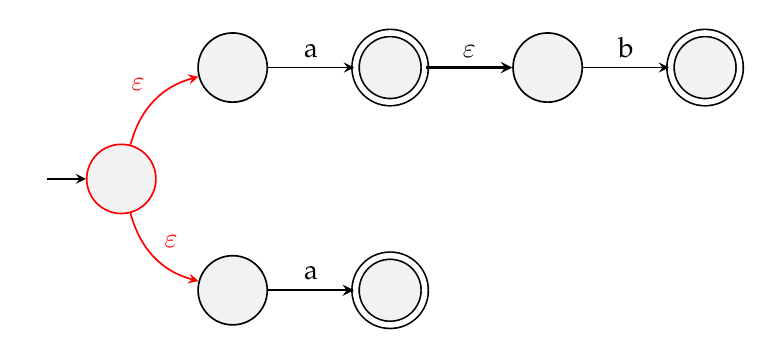
\begin{tikzpicture}
            \node[state, initial left, draw=red]                  (aba)   {};
            \node[state, above right of=aba]            (aq1)   {};
            \node[state, accepting, right of=aq1]       (aq2)   {};
            \node[state, right of=aq2]                  (bq1)   {};
            \node[state, accepting, right of=bq1]       (bq2)   {};
            \node[state, below right of=aba]            (aq3)   {};
            \node[state, accepting, right of=aq3]       (aq4)   {};
            \coordinate (x) at (aq2);
            \draw   (aq1) edge[]        node{a} (aq2)
                    (bq1) edge[]        node{b} (bq2)
                    (aq2) edge[thick]   node{$\varepsilon$} (bq1)
                    (aq3) edge[thick]   node{a} (aq4)
            ;
            \draw[red, thick]
                    (aba) edge[bend left]        node{$\varepsilon$} (aq1)
                    (aba) edge[bend right]        node{$\varepsilon$} (aq3)
            ;
        \end{tikzpicture}
    \end{minipage}
    
    %--- Page 2 --------------------------------------------------------------------
    \newpage    

    

    %--- Page 3 --------------------------------------------------------------------
    \newpage

	
    %--- Page 4 --------------------------------------------------------------------
    \newpage
    


    %--- Page 5 --------------------------------------------------------------------
    \newpage
    
    

    %--- Page 6 --------------------------------------------------------------------
    \newpage


\end{document}
